\documentclass[italian,10pt,a4paper]{report}
\usepackage[T1]{fontenc}
\usepackage{graphicx}
\usepackage{mathtools}
\usepackage{amssymb}
\usepackage{amsthm}
\usepackage{thmtools}
\usepackage[dvipsnames]{xcolor}
\usepackage{nameref}
\usepackage{babel}
\usepackage{hyperref}
\usepackage{cancel}
\usepackage{xspace}
\usepackage{cleveref}
\usepackage{mdframed}
\usepackage{minted}
\usepackage{listings}
\graphicspath{{img/theory/}}
%\usepackage{generictoolbox}
%% Qui copierai la definizione di generictoolbox
\newtheorem{definition}{Definizione}
\newtheorem{theorem}{Teorema}
\newtheorem{demonstration}{Dimostrazione}
\newtheorem{lemma}{Lemma}
\newcommand{\pbc}[1]{\mathbb{#1}}
\newcommand{\yes}{\textit{yes}}
\newcommand{\ve}{\,\vee\,}
\newcommand{\ive}{\,\wedge\,}
\newcommand{\polytime}{\textit{polytime}}
\newcommand{\tc}{\,\colon\,}
\newcommand{\np}{\text{NP}}
\newcommand{\npc}{\text{NPC}}
\newcommand{\p}{\text{P}}
\newcommand{\ipb}[1]{\mathcal{I}(\pbc{#1})}
\newcommand{\notexists}{\,\cancel{\exists}\,}
\newcommand{\onlyexists}{!\exists}
\newcommand{\n}{\mathbb{N}}
\newcommand{\z}{\mathbb{Z}}
\newcommand{\rs}{\mathbb{R}}
\newcommand{\cs}{\mathbb{C}}
\newcommand{\exps}{\textit{EXP}}
\newcommand{\no}{\textit{no}}
\newcommand{\problem}[3]{
	\begin{mdframed}[frametitle=\textbf{#1},frametitlerule=true]
		\textbf{Input:}\hspace{0.5\parindent}#2\\
		\textbf{Output:}\hspace{0.5\parindent}#3
	\end{mdframed}
}
\newcommand{\red}[1]{{\color{Red}#1}}
\newcommand{\green}[1]{{\color{Green}#1}}



\title{Manuale per la preparazione all'esame di complessità}
\author{Riccardo Torre}
\begin{document}
	\maketitle
	\chapter{Appunti delle lezioni}
	\chapter{Riduzioni}
	\section{Riduzioni}
\begin{definition}[Riduzione polinomiale tra problemi (alla Karp)]
	Un problema $\pbc{A}$ si riduce polinomialmente (alla Karp) a $\pbc{B}$ e si scrive $\pbc{A}\preceq\pbc{B}$ se $\exists$ un algoritmo polinomiale $f$ tale che \[\forall x \in \pbc{A}\tc \pbc{A}(x)=\yes \iff \pbc{B}(f(x))=\yes\] 
	L'effetto di $f$ è
	\[\underbracket{|x|}_{\substack{\textit{istanza}\\\textit{di $\pbc{A}$}}}\xlongrightarrow{\textit{effetto di }f}\underbracket{|y|}_{\substack{\textit{istanza}\\\textit{di $\pbc{B}$}}}\in O(|x|^c)\ive y=f(x)\]
	in tempo $O(|y|^d)$ si risponde \[\boxed{\pbc{B}(y)=\yes\iff\pbc{A}(x)=\yes}\] in tempo $O(|x|^c)+O(|y|^d)$, che è polinomiale.
\end{definition}
\subsection{Riduzione k-col a k+1-col}
Un grafo $G$ è propriamente colorato se \[\forall (u,v)\in E(G)\tc u\ne v \ive colore(v)\ne colore(u)\]
\begin{demonstration}
	\begin{figure}[thbp]
		\centering
		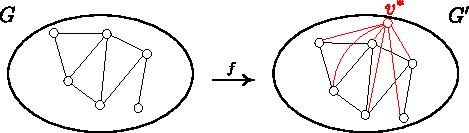
\includegraphics{k-coloring/k-coloring.pdf}
		\caption{riduzione k-coloring a k+1-coloring.}
		\label{fig:k-coloring}
	\end{figure}
	Fornire la funzione polytime $f$ tale che se $\forall G$ è $k-col$ allora \[G\ \textit{è k-colorabile}\iff f(G)\ \textit{è k+1-colorabile}\]
	
	$f$ è \textit{polytime computable}. Se $G$ è $k-col$ allora $G'$ è $k+1-col$. 
	\begin{itemize}
		\item quando viene colorato $G'$ per i vertici che erano in $G$ si tiene la k-colorazio-ne che era presente e per $v^\ast$ viene utilizzato il colore in più; 
		\item se $G'$ è k+1-col \textit{wlog\footnote{without loss of generality.}} si imposta a $k+1$ il colore in $v^\ast$. Poiché $\forall v\ne v^\ast$ $(v,v^\ast)\in E(G')$ si ha che $colore(v)\ne k+1$ e $colore(v)\in\{1,\dots,k\}$
		\item se $\forall v,w\in V(G)\tc e=(v,w) \ive colore(v)\ne colore(w)$ allora la colorazione è propria per $G$.
	\end{itemize}
	Per dimostrare l'implicazione inversa, basta partire da $G'$ e mostrare che il risolutore restituisce \textit{yes} per $k+1-col$, togliere $v^\ast$ e gli archi che lo congiungono, togliere il $k+1$ colore e mostrare che anche il risolutore di $k-col$ restituisce \textit{yes}.
	\qed
\end{demonstration}

Da $k-col\preceq k+1-col$ segue che
\begin{gather*}
	\exists f\tc G\to G'=f(G)\ive |G'|=|G|^c_f\quad [polytime]
\end{gather*}
Se esiste $A$ per $k+1-col$ $A(G)=k+1-col$ e $T_A(G')=O(|G'|^c_a)\implies B(G)=A(f(G))$ $B$ è un algoritmo \textit{polytime} per $k-col$. Il tempo di $B$ su $G$ è
\[T_B(G)=O(|G|^c_d)+T_A(f(G))=O(|G|^c_d)+O((|G|^c_d)^c_A)=O(|G|^{c_d\cdot c_A})\]

\subsubsection{Alcune osservazioni}
\begin{gather*}
	\pbc{A}\preceq\pbc{B} \ive \pbc{B}\in\p\implies \pbc{A}\in\p\\
	\pbc{A}\preceq\pbc{B}\ive \pbc{A}\notin\p\implies \pbc{B}\notin\p
\end{gather*}

Se $k-col\notin\p$ allora $B$ non può esistere. Questo implica che $A$ non può esistere e $k+1-col\notin\p$.

Si supponga che esista $\pbc{B}$ tale che \[\forall \pbc{A}\in \np\quad\pbc{A}\preceq\pbc{B}\]
\begin{figure}[thbp]
	\centering
	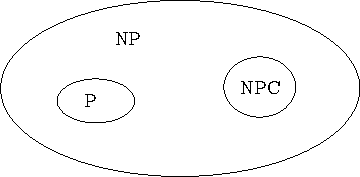
\includegraphics{p-np-npc/p-np-npc.pdf}
	\caption{relazioni tra le classi di complessità.}
	\label{fig:p-np-npc}
\end{figure}
\begin{itemize}
	\item Se $\pbc{B}\in\p$ allora $\pbc{A}\in\p$. Segue che $\forall \pbc{A}\in \np$ risulta $\np\subseteq \p\implies \p=\np$
	\item Se $\p\ne \np\implies B\notin\p$
\end{itemize}
\begin{definition}[NP-completezza]
	Si dice che $\pbc{B}$ è NP-completo ($\npc$) se 
	\begin{itemize}
		\item $\pbc{B}\in \np$
		\item $\forall \pbc{A}\in \np\tc \pbc{A}\preceq\pbc{B}$ ovvero $\pbc{B}$ è NP-hard
	\end{itemize}
\end{definition}
\subsection{Problemi NPC}
Esistono problemi NP-completi. Se $\pbc{A}\in\np$ se esiste un verificatore $B(\cdot,\cdot)$ ploytime per $\pbc{A}$ tale che \[\forall x \in \ipb{A}\tc\pbc{A}(x)=\yes\iff\exists y\tc B(x,y)=\yes\]
\subsection{Problema SAT (Satisfiability)}
\problem{SAT}{Formula CNF $\phi$}{$\yes\iff\phi$ è soddisfacibile}
\begin{definition}[Forumla CNF]
	Una formula è CNF\footnote{Conjunctive Normal Form.} se \[\phi(x_1\dots x_n)=\underbracket{C^1\ive C^2\ive\dots \ive C^n}_\textit{congiunzione di clausole}\] dove ogni $C^i\tc 1\le i\le n\ive l^i_j\tc 1\le j\le k$ \[C^i=\underbracket{l_1^i\ve l_2^i\ve\dots\ve l_k^i}_\textit{disgiunzione di letterali}\qquad l_j^i\in\{\underbracket{x_1,\dots,x_n,\overline{x_1},\dots,\overline{x_n}}_\textit{insieme di variabili\footnote{variabili true e false.}}\}\]
\end{definition}
\begin{definition}[Assegnamento]
	Un assegnamento $a$ è definito come\[a=(a_1,\dots,a_n)\in\{T,F\}^n\]
	Si dice che un assegnamento $a$ soddisfa $\phi$ se $\boxed{\phi(a_1,\dots,a_n)=T}$
\end{definition}
\subsection{Riduzione k-col a SAT}
Dato $G$ è possibile costruire in \textit{polytime} $\phi_G$ CNF tale che $G$ è k-colorabile se e solo se $\phi_G$ è soddisfacibile.

\paragraph{Dimensioni delle istanze}La taglia di G è\[|G|=|(V,E)|=|V|+|E|\] mentre quella di $\phi$ è \[|\phi|=n\] con $n$ il numero di letterali che sono contenuti all'interno di $\phi$.

\paragraph{Obbiettivo}L'obbiettivo che si vuole raggiungere è definire una funzione $f$ \textit{polytime computable} che permetta di ridurre le istanze del problema $k-col$ a istanze del problema SAT. In altre parole, dare una definizione di $k-col$ ridefinendo le sue istanze in maniera tale da utilizzare le istanze di SAT. Si definisce $\phi_G$ come 
\begin{equation}
	\boxed{\phi_G=\bigwedge_{v\in V}(C^v\ive D^v)\ive \bigwedge_{e\in E}E^e}\label{eqn:f-k-col-sat}
\end{equation}
tale che
\begin{align}
	\forall v\in V \tc&\begin{cases}
		C^v =x_1^v\ve x_2^v\ve\dots\ve x_k^v\\ D^v=\bigwedge_{1\le i \le j\le k}(\overline{x_i^v}\ve \overline{x_j^v})
	\end{cases}\label{eqn:sistema-vertici-kcol-sat}\\
	\forall e=(u,v)\in E\tc& E^e=\bigwedge_{1\le i\le k}(\overline{x_i^u}\ve \overline{x_i^v})\label{eqn:archi-kcol-sat}
\end{align}
dove \cref{eqn:sistema-vertici-kcol-sat} contiene due condizioni:
\begin{enumerate}
	\item ciascun vertice deve avere almeno un colore
	\item ciascun vertice non può contenere più di un colore
\end{enumerate}
che si traduce in ``\textit{ogni vertice deve avere esattamente un colore}''. La \cref{eqn:archi-kcol-sat} garantisce la colorazione propria del grafo. La definizione scelta permette di specificare in posizione apice di una variabile il vertice, e in posizione pedice il colore. La dimensione di $|\phi_G|$ diventa \[|\phi_G|=|V|\left(k+\binom{k}{2}2\right)+2k|E|\]
ovvero ciascun vertice dell'insieme $V$ ha una clausola $C^v$ lunga $k$ letterali, una clausola $D^v$ lunga 
per ogni coppia scelta di colori $\binom{k}{2}$ si hanno due letterali $\overline{x_i^v}$ e $\overline{x_j^v}$ e ciascun arco nell'insieme $E$ ha una clausola $E^e$ lunga 
per ogni possibile colore (i colori sono $k$), due letterali.
\subsubsection{Esempio}
Si estraggono le informazioni dal grafo
\begin{figure}[thbp]
	\centering
	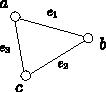
\includegraphics[width=0.3\linewidth]{k-col-sat/k-col-sat-graph-example}
	\caption{dal grafo si estraggono le informazioni per ricavare la formula CNF.}
	\label{fig:k-col-sat-graph-example}
\end{figure}
e si ricavano le equazioni
\begin{align*}
	C^a&=x_1^a\ve x_2^a \qquad  C^b=x_1^b\ve x_2^b \qquad C^c=x_1^c\ve x_2^c\\
	D^a&=\overline{x_1^a}\ve \overline{x_2^a} \qquad D^b = \overline{x_1^b}\ve\overline{x_2^b} \qquad D^c=\overline{x_1^c}\ve\overline{x_2^c}\\
	E^{e_1}&=(\overline{x_1^a}\ve\overline{x_1^b})\ive(\overline{x_2^a}\ve\overline{x_2^b})\\E^{e_2}&=(\overline{x_1^c}\ve\overline{x_1^b})\ive(\overline{x_2^c}\ve\overline{x_2^b})\\E^{e_3}&=(\overline{x_1^a}\ve\overline{x_1^c})\ive(\overline{x_2^a}\ve\overline{x_2^c})
\end{align*}
In questo caso i colori a disposizione sono 1 e 2 (pedice delle variabili). Il grafo non ha colorazione propria perché non si riesce a trovare una combinazione di colori sui vertici tale per cui \cref{eqn:archi-kcol-sat} è vera.
Si dimostra la riduzione.
\begin{demonstration}[$\implies$]
	Si assume $G$ k-colorabile. Sia $\{c(v)\tc v\in V\}$ una colorazione propria ovvero $\forall e=(u,v)\in E\tc c(u)\ne c(v)$ e con $c(v)\in\{1,\dots,k\}$. Si definisce l'assegnamento $a=(a^{v_1}_1,\dots, a^{v_1}_k,\dots, a^{v_n}_1,\dots,a^{v_n}_k)$ e si assegna 
	\begin{equation}
		a^{v_i}_j=\begin{cases}
			T & c(v_i)=j\\
			F & c(v_i)\ne j
		\end{cases}\label{eqn:assign-definition}
	\end{equation}
	Si mostra quindi che ogni gruppo di clausole è soddisfatto dall'assegnamento. Preso un $C^{|v|}(a)$\footnote{abuso di notazione, si immagini ci siano scritte tutte le variabili dell'assegnamento $a$.} si ha che l'assegnamento rende vera ogni clausola della \cref{eqn:f-k-col-sat}
	\begin{itemize}
		\item $C^v(a)=T$ perché per ogni vertice, in particolare per $v$, una variabile associata ha valore $T$ (esiste un legame tra il vertice e il colore per definizione di $a^{v_i}_j$);
		\item $D^v(a)=T$ perché nella definizione viene associato univocamente un valore alla variabile;
		\item $E^v(a)=T$ perché la colorazione è propria (poiché viene assunto che $G$ sia $k-col$ e che la colorazione associata a $G$ sia propria), ovvero $\forall e=(u,v)\tc c(u)\ne c(v)$. Se fosse $E^v(a)=F$ allora \[\exists i\tc \overline{x_i^u}\ve \overline{x_i^v}=F\implies x_i^u=T\ive x_i^v=T\implies a_i^u=T\ive a_i^v=T\]
		ma per la \cref{eqn:assign-definition} risulta $c(u)=i \ive c(v)=i \implies c(u)=c(v)$ in contraddizione con l'assunzione che la colorazione è propria.
	\end{itemize}
	concludendo che $\phi_G(a)=T$.\qed
\end{demonstration}
Per dimostrare la coimplicazione si parte da un assegnamento che rende vera una formula $\phi$ senza conoscere il grafo.
\begin{demonstration}[$\impliedby$]
	Si assume che $\phi_G(a)=T$ e si mostra che $G$ è $k-col$. L'assegnamento $a=(a_1^{v_1},\dots,a_n^{v_1},\dots,a_1^{v_n},\dots,a_n^{v_n})$ tale che $\phi_G(a)=T$. Si definisce una colorazione per $G$ basata su $a$:
	\[\forall v\in V\tc c(v)=i\iff a_i^v=T\]
	\begin{enumerate}
		\item ogni vertice ha un solo colore, infatti se $\phi(a)=T$ segue che:
		\begin{itemize}
			\item $C^v(a)=T\implies\exists i \tc a_i^v=T \implies c(v)=i$
			\item $D^v(a)=T\implies \notexists i,j\tc a_i^v=T\ive a_j^v=T$
		\end{itemize}
		da cui \[\onlyexists i\tc c(v)=i\]
		\item ogni arco \textbf{non è monocromatico} ovvero $c(u)\ne c(v)$. Poiché $\phi(a)=T\implies E^e(a)=T\implies\notexists  i\tc a_i^u=T \ive a_i^v=T\implies c(u)\ne c(v)$.
	\end{enumerate}
	Da cui $G$ è $k-col$. \qed
\end{demonstration}
Dunque $k-col\preceq SAT$.
\begin{figure}[thbp]
	\centering
	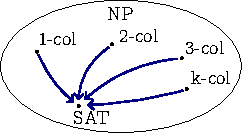
\includegraphics{k-col-sat/sat-is-npc}
	\caption{tutti i problemi k-col si riducono a SAT. Si vedrà che tutti i problemi si riducono a SAT.}
	\label{fig:sat-is-npc}
\end{figure}
\subsection{Problema Circuit-SAT}
\begin{figure}[thbp]
	\centering
	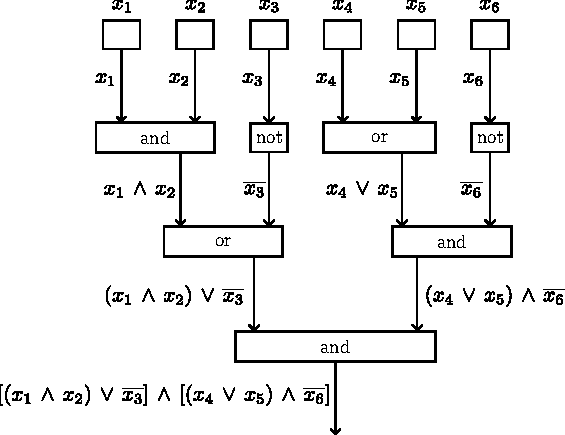
\includegraphics[]{circuit-sat/circuit-sat.pdf}
	\caption{circuito booleano.}
	\label{fig:circuit-sat}
\end{figure}
\problem{Circuit-SAT}{Circuito booleano $C$}{$\yes\iff C$ è soddisfacibile}
\begin{definition}[Circuito booleano]
	È un grafo aciclico diretto in cui ogni vertice ha un in-degree=1,2 tranne i vertici di input che hanno un in-degree=0.
	
	Ogni vertice ha un out-degree=1 e ha associato un \textbf{operatore booleano} \textit{and}, \textit{or}, \textit{not}. In particolare \textit{not} è associato a tutti i vertici con in-degree=1 mentre \textit{and} e \textit{or} a quelli con in-degree=2.
\end{definition}
Dato un assegnamento in input a $x_1,\dots,x_n$ allora $C(x_1,\dots,x_n)=v$ con $v$ valore dell'arco in output. Nell'esempio in \cref{fig:circuit-sat} si ha $C(0,1,1,1,1,1)=0$.
\subsection{Teorema di Cook-Levin}
\begin{theorem}[Cook-Levin]
	SAT è NP-completo\label{thm:cook-levin}
\end{theorem}
Per dimostrare il \cref{thm:cook-levin} si deve dimostrare che ($\color{Green}\checkmark$ = già dimostrato)
\begin{itemize}
	\item $\text{SAT}\in \np$ $\color{Green}\checkmark$
	\item $\text{Circuit-SAT}\preceq \text{SAT}$
	\item Circuit-SAT è NP-completo
	\begin{itemize}
		\item $\text{Circuit-SAT}\in\np$ $\color{Green}\checkmark$
		\item Circuit-SAT è NP-hard \[\forall\pbc{A}\in\np\tc\pbc{A}\preceq \text{Circuit-SAT}\]
	\end{itemize}
\end{itemize}
\begin{lemma}
	Per ogni problema $\pbc{B}\in\p$ e per ogni $n\in\n$\[\exists C_n\tc\forall x\in \ipb{B}\quad |x|=n \ive C_n(x)=\pbc{B}(x)\]
	Inoltre $C_n$ è computabile in tempo \textit{polytime} ovvero $\exists c\tc O(|x|^c)$.\label{lemma:circuito-booleano-algo}
\end{lemma}
Il $\cref{lemma:circuito-booleano-algo}$ afferma che, fissato un input $x$ con $|x|=n$, un algoritmo $A$ può essere tradotto in un circuito booleano $C_n$ tale che \[A(x)=C_n(x)\]
\begin{demonstration}[Circuit-SAT è NP-hard]
	Affermare \[\forall\pbc{A}\in\np\tc\pbc{A}\preceq\text{Circuit-SAT}\]
	significa \[x\in\ipb{A}\xrightarrow[\textit{in}\ x]{\polytime}C_x^\pbc{A}\tc\pbc{A}(x)=\yes\iff C_x^\pbc{A}\ \textit{è soddisfacibile}\]
	Sostenere che $\pbc{A}\in\np$ implica che
	\[\exists B(x,y)\tc\forall x\in\ipb{A}\quad\ipb{A}(x)=\yes\iff\exists y\in\{0,1\}^{|x|^c}\]
	
	Fissato $x$, il problema associato al calcolo di $B(x,y)$ 
	\problem{Calcolo di $\mathbf{B(x,y)}$}{$y$}{$B(x,y)$}
	è in $\p$. Seguendo quanto riportato dal \cref{lemma:circuito-booleano-algo} si può affermare che \[\exists C_n^\pbc{A}\tc \forall y\quad |y|=n \quad C_n^\pbc{A}(y)=B(x,y)\] $C_n^\pbc{A}$ è calcolabile in polytime nell'input, quindi $O(n^d)=O(|y|^d)=O(|x|^{c\cdot d})$.
	\begin{align*}
		{\color{Red}x\in\ipb{A}\textit{ è yes }}&\iff \exists y \tc B(x,y)=\yes\\&\iff \exists y \tc C_n^\pbc{A}(y)=\yes\\&\iff C_n^\pbc{A}\ \textit{è un'istanza yes per Circuit-SAT}
		\\&\iff \color{Red}\textit{Circuit-SAT}(C_n^\pbc{A})=\yes
	\end{align*}
	da cui si ottiene \[x\in\ipb{A}\textit{ è yes }\iff \textit{Circuit-SAT}(C_n^\pbc{A})=\yes\]
	Quindi $\textit{Circuit-SAT}\preceq \textit{SAT}$\qed
\end{demonstration}

Si dimostra che Circuit-SAT $\preceq$ SAT facendo riferimento ad un circuito booleano arbitrario in \cref{fig:dim-circuitsat-to-sat}
\begin{figure}[thbp]
	\centering
	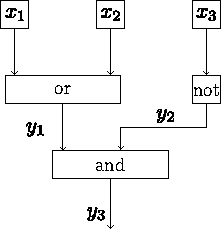
\includegraphics{circuit-sat/circuitsat-to-sat}
	\caption{circuito booleano della dimostrazione.}
	\label{fig:dim-circuitsat-to-sat}
\end{figure}
\begin{demonstration}[Circuit-SAT $\preceq$ SAT]
	\[\exists x \tc C(x)=T\iff \exists x'\tc \phi(x')=T\] Si pone $x_1\ve x_2=y_1$, $\overline{x_3}=y_2$ e $y_3=y_1\ive y_2$ da cui si ottiene la formula $\phi$ \[\phi(x_1,x_2,x_3,y_1,y_2,y_3)=[(x_1\ve x_2)=y_1]\ive[\overline{x_3}=y_2]\ive[y_3=y_1\ive y_2]\ive y_3\] 
	\paragraph{Osservazione} $a=b\equiv (\overline{a}\ve b)\ive(a\ve \overline{b})$
	
	Quindi \[\exists x \tc C(x)=T\iff\exists x,y\tc \phi(x,y)=T\]
	Si sa che $\forall\pbc{A}\in N\p\quad \pbc{A}\preceq\text{Circuit-SAT}\preceq\text{SAT}$
	\[x\rightarrow C_x^\pbc{A}\rightarrow\phi\]
	e dunque $\pbc{A}\preceq \text{SAT}$. SAT è NP-hard e appartiene alla classe $\np$. Dunque SAT è NP-completo.\qed
\end{demonstration}
\subsubsection{Dimostrare che un problema è NP-completo}
Per dimostrare che un problema $\pbc{D}$ è NP-completo basta mostrare che
\begin{itemize}
	\item $\pbc{D\in\np}$ facile perché basta mostrare che una soluzione è verificabile in tempo polinomiale;
	\item $\forall \pbc{A}\in\np\quad \pbc{A}\preceq\pbc{D}$ la si dimostra usando la transitività delle riduzioni. Si sceglie un problema $\pbc{B}\in\npc$ e si dimostra che $\pbc{B}\preceq\pbc{D}$. Poiché $\forall \pbc{A}\quad \pbc{A}\preceq\pbc{B} \ive \pbc{B}\in\npc\implies\forall \pbc{A}\quad \pbc{A}\preceq\pbc{D}$ (NP-hardness).
\end{itemize}	

\begin{definition}[k-CNF]
	Una formula k-CNF è una CNF in cui tutte le clausole hanno al più $k$ letterali.
\end{definition}
Si consideri la formula CNF
\begin{equation}
	\phi=\underbracket{(x_1\ve x_2\ve x_3)}_{C^1}\ive\underbracket{(x_1\ve\overline{x_2}\ve\overline{x_4}\ve x_5)}_{C^2}\ive \underbracket{(x_1\ve\overline{x_3}\ve \overline{x_4}\ve x_5\ve x_6)}_{C^3}\label{eqn:esempio-3-cnf}
\end{equation}
\problem{3-SAT}{3-CNF $\phi$}{$\yes\iff \phi$ è soddisfacibile}
\paragraph{Osservazione} $\text{2-SAT}\in\np$.
$\text{3-SAT}\in\np$ come per SAT. Si vuole dimostrare che 3-SAT è NP-completo, mostrando che 
\begin{align*}
	\text{SAT}&\preceq\text{3-SAT}\\
	\underbracket{\phi}_{\text{CNF}}&\rightarrow\underbracket{\phi'}_{\text{3-CNF}}
\end{align*}
Data una clausola $C$ che è formata da più di 3 letterali, si costruiscono le clausole $D_1,D_2,\dots,D_t$ con 3 letterali tale che $C$ è soddisfacibile $\iff D_1\ive D_2\ive\dots\ive D_t$ è soddisfacibile. Si supponga che \[C=l_1\ve l_2 \ve l_3\ve l_4\ve \dots\ve l_k\quad \textit{con}\quad k>3\]
dove $l_i\in\{x_1,\overline{x_1},\dots,x_n,\overline{x_n}\}$. La clausola CNF si può riscrivere come una 3-CNF
\[(l_1\ve l_2\ve z_1)\ive(\overline{z_1}\ve l_3\ve z_2)\ive (\overline{z_2}\ve l_4\ve z_3)\ive \dots\ive (\overline{z_{k-3}}\ve l_{k-1}\ve l_k)\]
e considerando la $\phi$ e passandola in forma 3-CNF diventa
\[C'=(l_1\ve l_2\ve z_1)\ive(\overline{z_1}\ve l_3\ve z_2)\ive (\overline{z_2}\ve l_4\ve z_3)\ive (\overline{z_3}\ve l_5\ve l_6)\]
che contiene clausole di taglia 3. 
Alcune osservazioni:
\begin{itemize}
	\item il numero dei letterali della nuova clausola $C'$ è meno del doppio di quella originale $C$;
	\item se $C$ è soddisfacibile, esiste un assegnamento che rende soddisfacibile anche la clausola $C'$. Quindi esiste un assegnamento che rende almeno un letterale vero. Usando la scelta che soddisfa $C$ che la rende vera, allora si usa la stessa scelta su $C'$ e conseguentemente deve risultare vera. 
\end{itemize}
Quindi per verificare che $C'$ è soddisfacibile se $C$ è soddisfacibile, si mostra che, dato un letterale che rende vera la clausola, indipendentemente dagli altri letterali, si pongono i valori di $z$ delle clausole vicine ad un valore che le rende vere. Questo genera un effetto ``a catena'' per cui si propaga la scelta a tutte le clausole tale che ciascuna risulterà vera.

Per mostrare la coimplicazione, si suppone che esista un assegnamento
\begin{gather*}
	\exists a_x,a_z\tc  ((l_1\ive l_2\ive z_1)=T \implies C'=T) \ive (a_x\textit{ rende vera } C)
\end{gather*}

Si suppone per assurdo che $a_x, a_z$ soddisfa $C'$ ma tutti gli $l_i$ sono falsi. Se $a_z$ rende $C'$ vero ma $a_x$ rende $C = F$, vuol dire che tutti gli $l_i$ sono falsi. Il problema è che se non è presente almeno un letterale vero, i soli $z$ non sono sufficienti a rendere vera $C'$. Per cui si arriva all'assurdo. Con il verde si indica il vero e con il rosso il falso.
\begin{gather*}
	(\red{l_1}\ve \red{l_2}\ve \green{z_1})\ive(\red{\overline{z_1}}\ve \red{l_3}\ve \green{z_2})\ive (\red{\overline{z_2}}\ve \red{l_4}\ve \green{z_3})\ive \dots\ive (\red{\overline{z_{k-3}}}\ve \red{l_{k-1}}\ve \red{l_k})
\end{gather*}

Tornando a considerare l'\cref{eqn:esempio-3-cnf} la formula $\phi'$ diventa
\begin{gather*}
	\phi'=(x_1\ve x_2\ve x_3)\ive(x_1\ve\overline{x_2}\ve z_1)\ive \underbracket{(\overline{z_1}\ve \overline{x_1}\ve x_5)}_{C^2}\ive\\
	\underbracket{(x_4\ve\overline{x_3}\ve z_2)\ive(\overline{z_2}\ive \overline{x_4}\ve z_3)\ive (\overline{z_3}\ve x_5\ve x_6)}_{C^3}
\end{gather*}


Anche questa versione di 3-SAT è NP-completa.
\problem{3-SAT (esattamente 3)}{una 3-CNF in cui tutte le clausole hanno taglia 3}{$\yes\iff\phi$ è soddisfacibile}
\begin{demonstration}[3-SAT esattamente 3 è NP-completo]
	Data una CNF $\phi$ con clausole da $\le 3$ letterali, possiamo creare una CNF $\varphi$ con clausole da 3 letterali tali che $\phi$ è soddisfacibile se e solo se $\varphi$ è soddisfacibile.
	
	\begin{gather*}
		\phi=C^1\ive C^2\ive\dots\ive C^n\\
		\begin{multlined}
			|C^1|=1\quad C^1=l\implies(l\ve z_1\ve z_2)\ive(l\ve\overline{z_1}\ve z_2)\ive(l\ve z_1\ve \overline{z_2})\ive\\(l\ve \overline{z_1}\ve\overline{z_2})\\
			|C^2=2|\quad C^2=l_1\ve l_2\implies (l_1\ve l_2\ve z_1)\ive (l_1\ve l_2\ve \overline{z_1})
		\end{multlined}
	\end{gather*}
\end{demonstration}


\begin{definition}[Riduzione polinomiale]
	$\pbc{A}$ è NP-completo e $\pbc{B}\in\np$ e \[\underbracket{\pbc{A}\preceq\pbc{B}\implies \pbc{B}\ \text{è NP-completo}}_{\text{$\pbc{B}$ è NP-hard}}\]
	
	Una riduzione da $\pbc{A}$ a $\pbc{B}$ ($\pbc{A}\preceq\pbc{B}$) permette di risolvere $\pbc{A}$ in \textit{polytime} se esiste un programma/algoritmo che risolve $\pbc{B}$ in \textit{polytime}.
\end{definition}
Si definisce un risolutore per $\pbc{A}(x)$
\begin{mdframed}[frametitlerule=true, frametitle={Risolutore per $\pbc{A}$}]
	\textbf{Input: }$x\in \ipb{A}$\\
	$y\gets Riduzione(x)$\\
	$\textbf{return}\ Solutore-\pbc{B}(y)$
\end{mdframed}
e la subroutine di riduzione
\begin{mdframed}[frametitle={Subroutine $\mathbf{Riduzione(x)}$},frametitlerule=true]
	\textbf{Input:} $x\in \ipb{A}$\\
	\textbf{Output:} $y\in\ipb{B}$
\end{mdframed}
\begin{figure}[thbp]
	\centering
	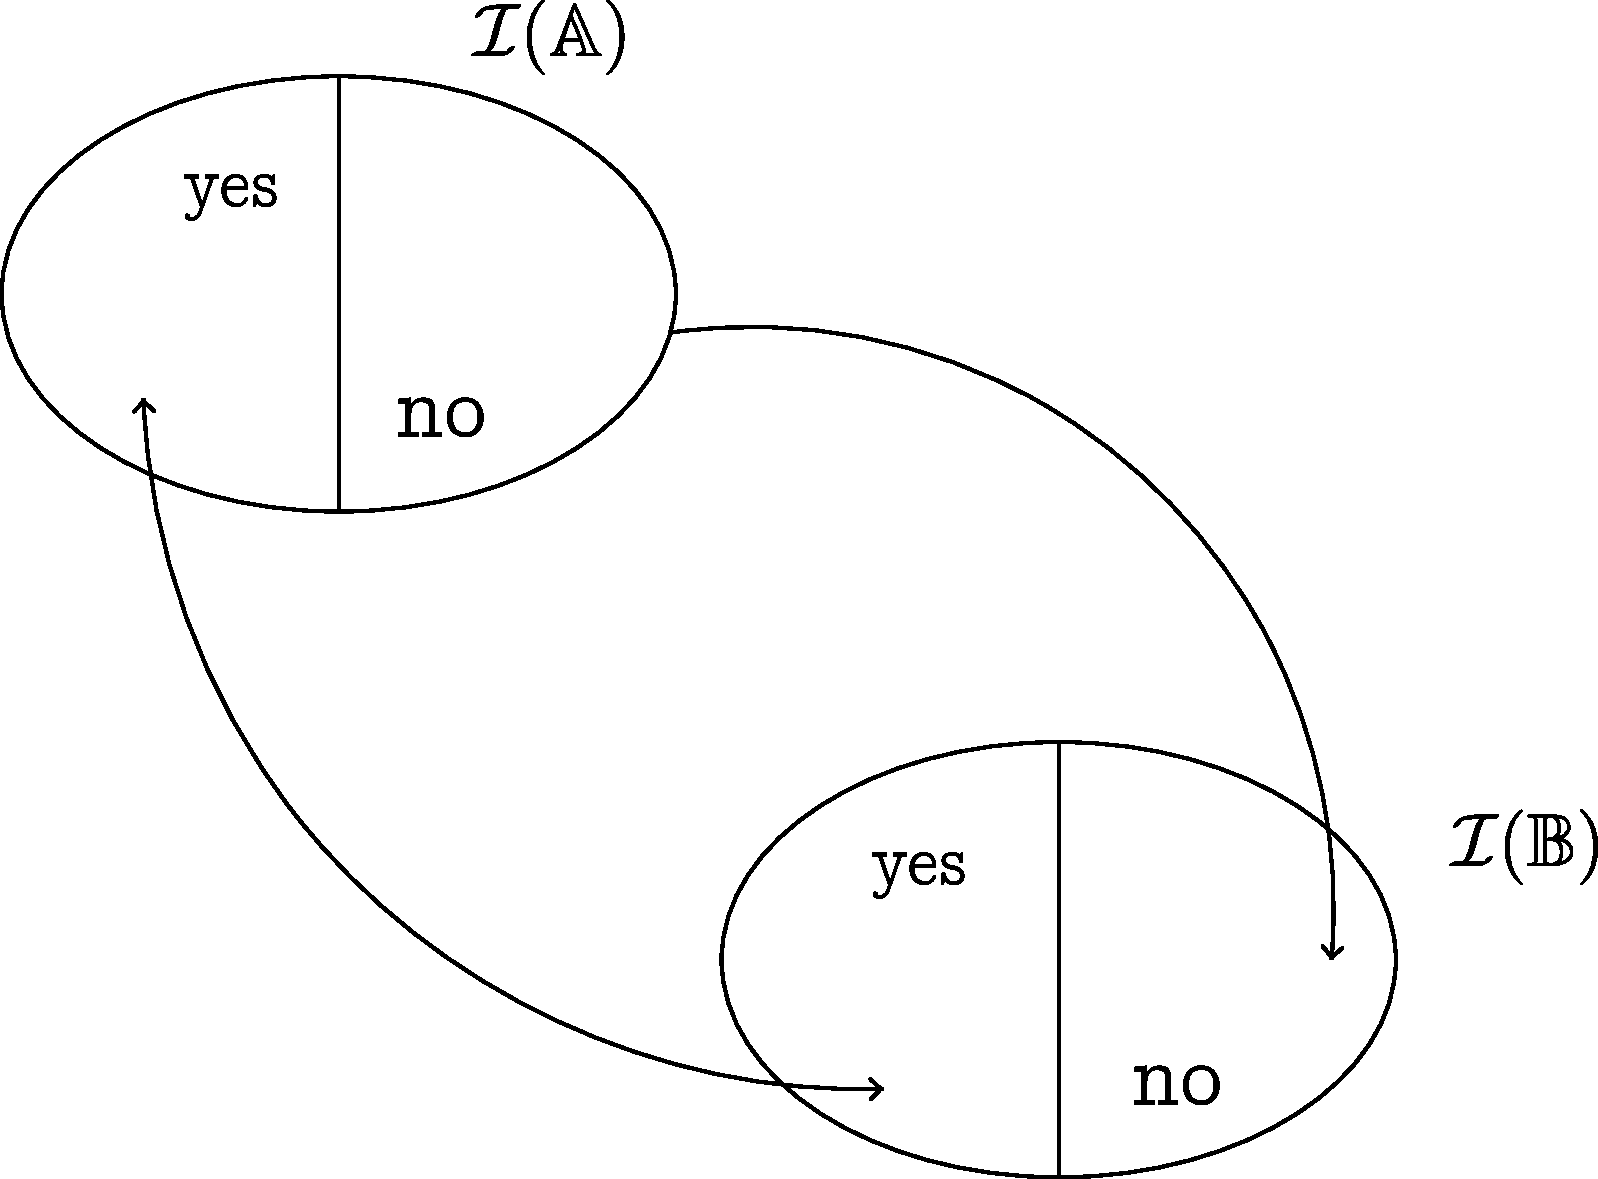
\includegraphics[width=0.7\linewidth]{dim-nae-3-sat-npc/riduzione.pdf}
	\caption{}
	\label{fig:}
\end{figure}


\subsection{NAE-k-SAT (Not all equal k-SAT)}
\problem{NAE-k-SAT (Not all equal k-SAT)}{formula k-cnf $\phi$}{$\yes\iff\phi$ NAE-soddisfa k-SAT (esiste un assegnamento $a$ tale che in ogni clausola $C^i$, $a$ pone almeno un letterale a $T$ e almeno uno a $F$)}
Si consideri l'assegnamento $\phi$
\begin{gather*}
	\phi(x_1,x_2,x_3)=(x_1\ve \overline{x_2}\ve x_3)\ive(\overline{x_1}\ve\overline{x_2}\ve\overline{x_3})
\end{gather*}
con $a=(x_1=T,x_2=F,x_3=T)$. Tale assegnamento non è NAE-soddisfacibile per $\phi$. L'assegnamento $b=(x_1=F,x_2=F,x_3=T)$ NAE-soddisfa $\phi$.
\paragraph{Osservazione} Data $\phi$, se $a=(a_1,\dots,a_n)$ NAE-soddisfa $\phi$ allora anche $\overline{a}=(\overline{a_1},\dots,\overline{a_n})$ NAE-soddisfa $\phi$. Inoltre \begin{equation*}
	\overline{a_i}=\begin{cases}
		F & a_i=T\\ T & a_i=F
		\end{cases}
\end{equation*}
NAE-3-SAT è NP-completo
\begin{enumerate}
	\item $\text{NAE-3-SAT}\in \np$: esiste un verificatore polinomiale $\color{Green}\checkmark$
	\item NAE-3-SAT è NP-hard: $\text{3-SAT}\preceq\text{NAE-4-SAT}\preceq\text{NAE-3-SAT}$. Si dà la dimostrazione in due parti.
\end{enumerate}
\begin{demonstration}[$\text{3-SAT}\preceq\text{NAE-4-SAT}$]
	Per dimostrare che 3-SAT si riduce a NAE-4-SAT si può costruire una subroutine che 
	\begin{equation*}
		\underbracket{\phi}_{\text{3-CNF}}\xlongrightarrow{R}\underbracket{\psi}_{\text{4-CNF}}
	\end{equation*}
	tale che $\phi\ \text{è soddifacibile}\ \iff \psi\ \text{è NAE-soddisfacibile}$. Ovvero
	\begin{align*}
		\underbracket{\exists a\tc\forall C^i\ \text{dentro}\ \phi\ \text{risulta}\ C(a)=T}_{\substack{\text{in $C(a)$ esiste un letterale true}}}\iff&\exists b\tc \forall D^i\ \text{dentro}\ \psi\ D(i)^b\ \text{contiene}\\&\text{un letterale true e un letterale false}
	\end{align*}
	Si supponga di avere la formula \[\phi(x_1,x_2,x_3)=\underbracket{(x_1\ve x_2\ve \overline{x_3})}_{C^1}\ive\underbracket{(\overline{x_1}\ve\overline{x_2}\ve \overline{x_3})}_{C^2}\] Data la riduzione $R$ e $\phi=(x_1,\dots,x_n)=\bigwedge_{i=1}^n C^i$ crea $\psi=(x_1,\dots,x_n,z)$. Allora \[\psi(x_1,\dots,x_n,z)=\bigwedge_{i=1}^nD^i\] dove ogni \[D^i=C^i\ve z\] Ad esempio \[\psi(x_1,x_2,x_3,z)=\underbracket{(x_1\ve x_2\ve x_3\ve z)}_{D^1}\ive\underbracket{(\overline{x_1}\ve\overline{x_2}\ve\overline{x_3}\ve z)}_{D^2}\]
	Si osserva che $R$ è polytime. Adesso si vuole dimostrare la coimplicazione. 
	\begin{itemize}
		\item[$\implies$] Si supponga che \[\exists a=(a_1,\dots,a_n)\tc \forall i C^i(a)=T\implies b=(a_1,\dots,a_n,F)\] da cui $b$  NAE-soddisfa $\psi$ \qed
		\item[$\impliedby$] Si supponga che \[\exists b=(b_1,\dots,b_n,b_{n+1})\tc \forall D\ D^i(b)\ \text{contiene un letterale vero e uno falso}\] Allora si può assumere che $D^i(b)$ è del tipo $(l_1\ve l_2 \ve l_3\ve z)$ con $z=F$ e almento uno tra $l_1,\dots,l_n$ è posto a $T$. Se $z=T$ allora basterà invertirlo con uno di quelli tra gli $l_1,\dots,l_n$ posti a $F$ e metterlo nella posizione della $z$. \[D^i(\underbracket{b_1,\dots,b_n}_{l_1,\dots,l_n},\underbracket{b_{n+1}}_z)=(\underbracket{b_1,\dots,b_n}_T,\underbracket{b_{n+1}}_F)\implies C(b_1,\dots,b_n)=T\] da cui $\exists a=(b_1,\dots,b_n)$ che soddisfa $\phi$ \qed 
	\end{itemize}
	quindi è stato dimostrato che $\text{3-SAT}\preceq \text{NAE-4-SAT}$
	\qed
\end{demonstration}

\begin{demonstration}[$\text{NAE-4-SAT}\preceq\text{NAE-3-SAT}$]
	Si vuole mostrare come trasformare una formula $\psi$ in una formula $\varphi$
	\begin{equation*}
		\underbracket{\psi}_{\text{NAE-soddif.}} \longrightarrow \underbracket{\varphi}_{\text{NAE-soddif.}}
	\end{equation*}
	Si supponga che $\psi=C^1\ive C^2\ive\dots\ive C^n=\bigwedge_{i=1}^nC^i$ e ogni $C^4=l_1\ve l_2\ve\dots\ve l_4$. L'idea è di generare da $C^4$ due clausole $C^{i,1}=l_1\ve l_2\ve z^i$ e $C^{i,2}=l_3\ve l_4\ve \overline{z^i}$. La formula $\varphi=\bigwedge_{i=1}^m C^{i,1}\ive C^{i,2}$. La formula \[\psi={\color{Red}(x_1\ve x_2\ve x_3\ve \overline{x_4})}\ive{\color{Blue}(\overline{x_1}\ve x_2\ve \overline{x_3}\ve x_4)}\] diventa \[\varphi={\color{Red}(x_1\ve x_2\ve z^1)\ive (x_3\ve \overline{x_4}\ve\overline{z^1})}\ive{\color{Blue}(\overline{x_1}\ve x_2\ve z^2)\ive(x_3\ve x_4\ve \overline{z^2})}\] Si dimostra che $\exists a\ \text{per}\ \psi\implies\exists b\ \text{per}\ \varphi$. Infatti, dato che l'assegnamento $l_1,\dots,l_4$ NAE-soddisfa $\psi$, le coppie $l_1\ve l_2$ e $l_3\ve l_4$ sono o nella configurazione di due letterali con stesso valore e due con uno diverso, oppure tutti con valore diverso. Dunque si può scegliere una configurazione per le $z$ che NAE-soddisfa $\varphi$.
	
	Si dimostra adesso che $\exists b\ \text{per}\ \varphi \implies\exists a\ \text{per}\ \psi$. Per assurdo se si scegliesse un assegnamento indipendentemente dall'essere o non essere NAE-soddisfacibile
		\[\psi={\color{Red}(\utrue{x_1}\ve \utrue{x_2}\ve \utrue{x_3}\ve \utrue{\overline{x_4}})}\ive{\color{Blue}(\ufalse{\overline{x_1}}\ve \ufalse{x_2}\ve \ufalse{\overline{x_3}}\ve \ufalse{x_4})}\]
	si arriverebbe ad avere un assurdo (le $z$ e la loro negazione non possono avere stesso valore)
	\[\varphi={\color{Red}(\utrue{x_1}\ve \utrue{x_2}\ve \ufalse{z^1})\ive (\utrue{x_3}\ve \utrue{\overline{x_4}}\ve\ufalse{\overline{z^1}})}\ive{\color{Blue}(\ufalse{\overline{x_1}}\ve \ufalse{x_2}\ve \utrue{z^2})\ive(\ufalse{x_3}\ve \ufalse{x_4}\ve \utrue{\overline{z^2}})}\]
	e dunque necessariamente l'assegnamento $b$ deve porre per ciascuna clausola almeno un letterale vero e uno falso.
	\qed
\end{demonstration}
NAE-3-SAT è NP-completo.

\paragraph{Esercizio} Provare che $\text{k-SAT}\preceq\text{NAE-k-SAT}$. L'idea è di ripetere la dimostrazione facendo vedere che $\text{k-SAT}\preceq\text{NAE-(k+1)-SAT}$ e che $\text{NAE-(k+1)-SAT}\preceq \text{NAE-k-SAT}$.
\begin{demonstration}[$\text{NAE-3-SAT}\preceq\text{3-col}$]
	
	Si vuole dimostrare adesso che $\text{NAE-3-SAT}\preceq\text{3-col}$ e dunque che \[\phi\xlongrightarrow{R}G_\phi(V,E)\] Avendo $\phi=C^1\ive C^2\ive\dots\ive C^n$ dove ogni $C^i=l_1^i\ve l_2^i\ve l_3^i$ si può costruire un grafo $G$ nel seguente modo
	\subsubsection{Codifica dei letterali}
	\begin{itemize}
		\item si collega ciascun vertice contenente un $x_i$ con il proprio negato $\overline{x_i}$;
		\item si collegano i vertici al vertice $v$;
		\item si associa il colore rosso ai vertici a cui corrispondono letterali con valore falso e il colore blu a quelli a cui corrispondono letterali con valore vero;
		\item si associa il verde al vertice rimanente in $G$.
	\end{itemize}
	\subsubsection{Codifica delle clausole}
	\begin{itemize}
		\item si creano dei grafi $G_{C_i}$ che rappresentano le clausole. Ciascun letterale deve essere collegato con quello opposto contenuto in $G$. Nella \cref{fig:rgb-graph} $C_i = x_1 \ve \overline{x_2}\ve x_3$;
		\item si colorano due vertici con i colori blu e rosso (blu per i vertici true e rosso per i vertici false) e il terzo vertice viene colorato di verde per mantenere sia $G$ che $G_{C_i}$ propriamente colorati.
	\end{itemize}
	\begin{figure}[thbp]
		\centering
		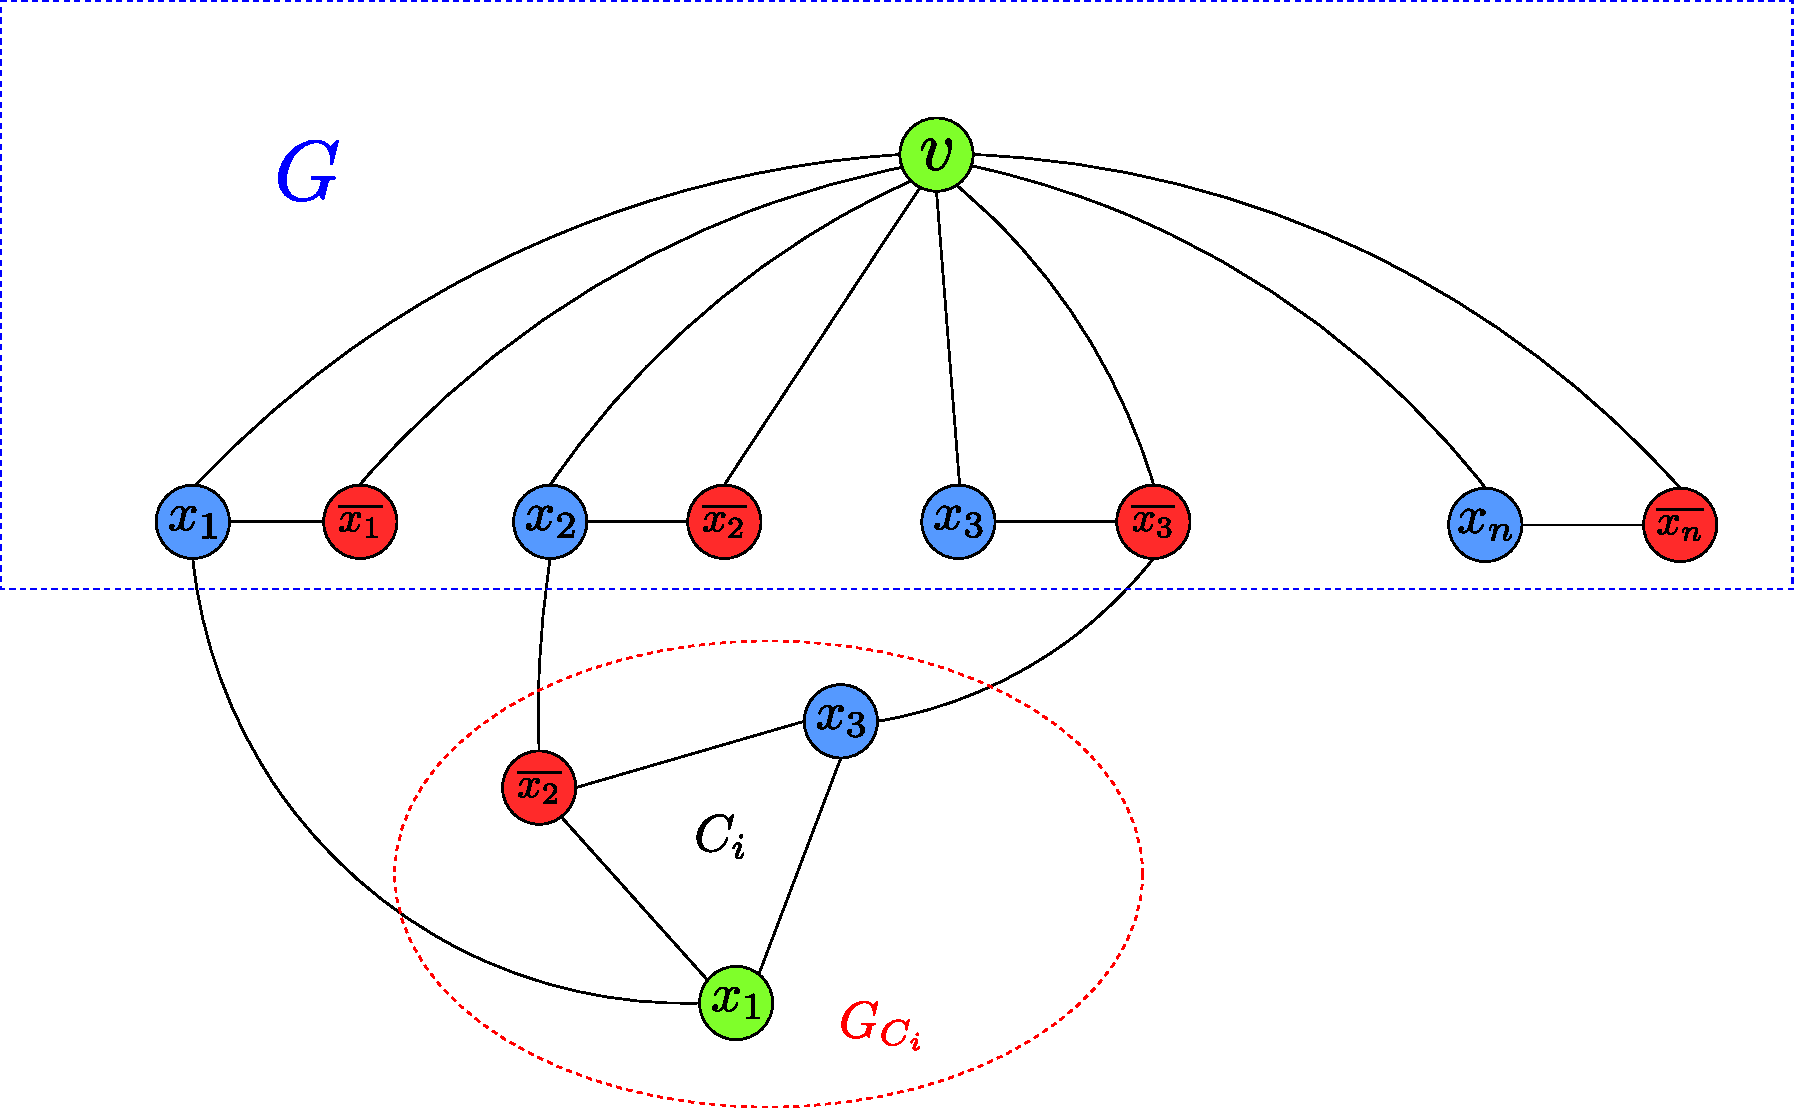
\includegraphics[width=\linewidth]{nae-3-sat-to-3-col/nae-3-sat-3-col}
		\caption{grafo 3-col.}
		\label{fig:rgb-graph}
	\end{figure}
	\paragraph{Polinomialità della riduzione}La riduzione è polinomiale. Se la formula ha $3m$ letterali, il grafo ha $3m+2n+1$ vertici, dove $3m$ sono il numero di vertici di tutti i grafi $G_{C_i}$, $2n$ sono il numero di vertici blu e rossi che compongono $G$ e $1$ è il vertice verde di $G$. Il numero degli archi è  $2n+n+3m+3m$ dove $2n$ sono quelli che partono dal vertice verde, $n$ sono quelli che collegano vertici di colore blu a quelli di colore rosso di $G$ e $3m$ gli archi che congiungono i grafi $G_{C_i}$ con $G$ e $3m$ che compongono i grafi $G_{C_i}$.
	\begin{demonstration}[$\implies$]
		Si dimostra che 
		\begin{gather*}
			\phi\ \text{è NAE-soddif.}\ \implies\exists a=(a_1,\dots,a_n)\in\{T,F\}^n \tc\forall i\ C^i(a)\ \text{contiene}\\\text{un letterale T e uno F e}\ \exists j,k\tc l^i_j(a)=T\ive l^i_k(a)=F
		\end{gather*}
		Si definisce una colorazione per un vertice (a cui si associa un letterale) come 
		\begin{gather*}
			c(w)=\begin{cases}
				B&\text{se $w$ è etichettato con $l_i$ e $l_i(a)=T$}\\
				R&\text{se $w$ è etichettato con $l_i$ e $l_i(a)=F$}
			\end{cases}
		\end{gather*}
		e $c(v)=G$. Si osserva che il grafo $G$ è propriamente colorato per costruzione. Gli archi che collegano i vertici di $G$ e $G_{C_i}$ sono propriamente colorati. Gli archi dei grafi $G_{C_i}$ per la NAE-soddisfacibilità di ciascuna clausola e per come sono stati costruiti sono propriamente colorati.\qed
	\end{demonstration}
	\begin{demonstration}[$\impliedby$]
		Siano i grafi $G$ e $G_{C_i}$ propriamente colorati. Si mostra che, scelto un assegnamento di colori per $G$ tale da renderlo propriamente colorato, esiste un assegnamento che collega i due grafi che è propriamente colorato. Si mostra che la colorazione segue quella di $G_{C_i}$. Infine si mostra che la colorazione di $G_{C_i}$ corrisponde ad una clausola $C_i$ che è NAE-soddisfacibile.\qed
	\end{demonstration}
	questo chiude la dimostrazione. \qed
\end{demonstration}
\end{document}